% Pagina originale 36
\pagina{36}
\[
\tan\theta=\frac{NH}{PH},\qquad
\tan\theta'=\frac{NH}{QH},\qquad
\tan\alpha=\frac{NH}{CH}.
\]
\[
\theta\simeq\tan\theta\simeq\frac yp,\qquad
\theta'\simeq\tan\theta\simeq\frac yq,\qquad
\alpha\simeq\tan\alpha\simeq\frac yR.
\]
\[
\theta+\theta'=2\alpha\quad\Longrightarrow\quad
\frac yp+\frac yq=\frac{2y}{R}
\quad\Longrightarrow\quad \frac1p+\frac1q=\frac2R.
\]
\subsubsection*{Specchio concavo: fuoco}
\begin{center}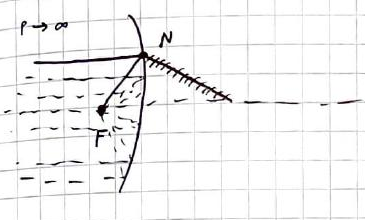
\includegraphics[width=.45\linewidth]{ottica_tex_assets/b36_p36_1.png}\end{center}
\[
P\longrightarrow\infty\quad\Longrightarrow\quad
p\longrightarrow\infty\quad\Longrightarrow\quad\frac1p\longrightarrow0,
\qquad
\frac1p+\underbrace{\frac1q}_{1/f}=\frac2R
\quad\Longrightarrow\quad f=\frac R2.
\]
Per il principio di invertibilità del raggio luminoso, qualunque raggio che parte dal fuoco, dopo aver colpito lo specchio, viene riflesso parallelamente all'asse. Cambiando verso di percorrenza il percorso rimane invariato, solo percorso nel verso opposto ma identico:
\[
p=f\quad\Longrightarrow\quad q\longrightarrow\infty.
\]
Se $P\in(F,V)$ i raggi divergeranno.
\begin{center}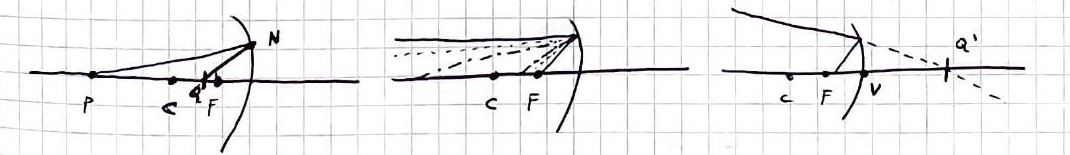
\includegraphics[width=\linewidth]{ottica_tex_assets/b36_p36_2.png}\end{center}
È il prolungamento del raggio ad intersecarsi con le superficie. Si parla in questo caso di \emph{immagine virtuale}.
\[
\frac1p-\frac1q=\frac2R.
\]
% Nella seconda approssimazione la scansione scrive tan(theta) anziché tan(theta').
% Pagina originale 37
\pagina{37}
\subsubsection*{Specchio convesso}
\begin{center}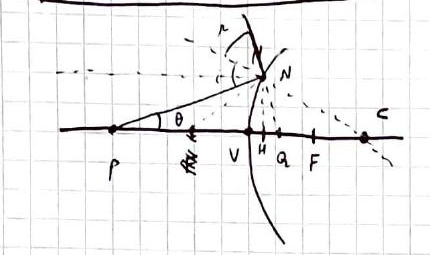
\includegraphics[width=.5\linewidth]{ottica_tex_assets/b36_p37_1.png}\end{center}
\[
i=\theta+\alpha,\qquad \theta'=r+\alpha
\quad\Longrightarrow\quad\theta'-\theta=2\alpha.
\]
\[
\tan\theta=\frac{NH}{PH},\qquad
\tan\theta'=\frac{NH}{QH},\qquad
\tan\alpha=\frac{NH}{CH},\qquad
 y=NH,\quad p=PH,\quad q=QH.
\]
\[
\theta\simeq\tan\theta,\qquad\theta'\simeq\tan\theta',\qquad
\alpha\simeq\tan\alpha.
\]
\[
\frac yq-\frac yp=\frac{2y}{R}
\quad\Longrightarrow\quad\frac1q-\frac1p=\frac2R
\qquad\left(\frac1p-\frac1q=-\frac2R\right).
\]
\[
p\longrightarrow\infty\quad\Longrightarrow\quad f=\frac R2.
\]
Nello specchio convesso l'immagine è sempre virtuale.
\subsubsection*{Convenzione dei segni}
\begin{center}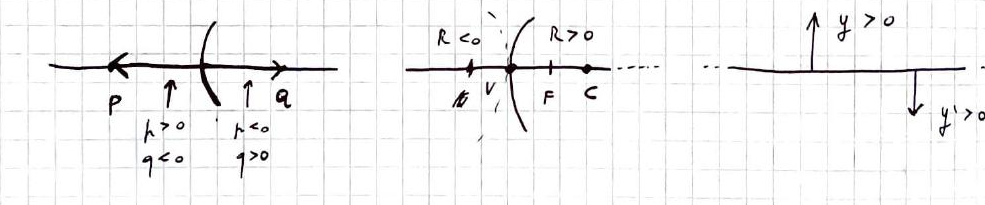
\includegraphics[width=\linewidth]{ottica_tex_assets/b36_p37_2.png}\end{center}
A sinistra del vertice: $p>0$, $q<0$; a destra: $p<0$, $q>0$.
$R<0$ a sinistra, $R>0$ a destra. Sopra l'asse $y>0$; sotto l'asse nel disegno è indicato $y'>0$.
% Il disegno originale riporta y'>0 sotto l'asse; etichetta conservata.
\[
\frac1{|p|}+\frac1{|q|}=\frac2{|R|},\qquad
\frac1{|p|}-\frac1{|q|}=\frac2{|R|},\qquad
\frac1{|p|}-\frac1{|q|}=-\frac2{|R|}.
\]
\[
\boxed{\frac1p-\frac1q=-\frac2R}.
\]
\begin{center}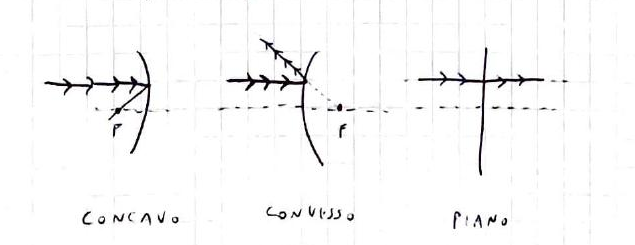
\includegraphics[width=.85\linewidth]{ottica_tex_assets/b36_p37_3.png}\end{center}
Specchio concavo, convesso, piano.
% Pagina originale 38
\pagina{38}
\subsubsection*{Costruzione dell'immagine}
\begin{center}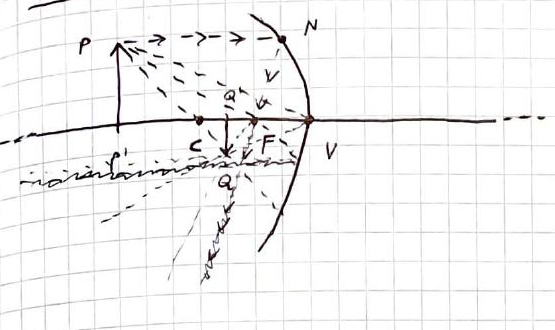
\includegraphics[width=.65\linewidth]{ottica_tex_assets/b36_p38_1.png}\end{center}
Ci sono quattro raggi notevoli:
\begin{enumerate}
\item $P\to N\to F$;
\item $P\to F\to\infty$;
\item $P\to C$;
\item $P\to V$.
\end{enumerate}
Dove si intersecano i quattro raggi notevoli si trova $Q$ ($Q'$ è la proiezione sulla superficie).
\subsubsection*{Ingrandimento trasversale}
\[
I_y=\frac{y'}y=\frac{QQ'}{PP'}.
\]
\[
\begin{gathered}
I_y>1\quad\text{(immagine ingrandita)},\\
I_y<1\quad\text{(immagine rimpicciolita)},\\
I_y=1\quad\text{(immagine coincidente)}.
\end{gathered}
\]
\begin{align*}
I_y&=\frac{QQ'}{PP'}=\frac{CQ}{CP}
=\frac{|R|-|q|}{p-|R|}=\frac{-R+q}{p+R}\\
&=-\frac qp\left(\frac{R/q-1}{1+R/p}\right),\\
\frac1p-\frac1q&=-\frac2R
\quad\Longrightarrow\quad\frac Rp=\frac Rq-2
\quad\Longrightarrow\quad1+\frac Rp=\frac Rq-1,\\
I_y&=-\frac qp\cdot1=-\frac qp.
\end{align*}
\[
I=-\frac qp.
\]
In questo caso $p>0$, $q<0$, quindi $I>0$.
Se $I>0$ l'immagine è capovolta. Se $I<0$ l'immagine è dritta.
% Pagina originale 39
\pagina{39}
\subsubsection*{Specchio piano}
\begin{center}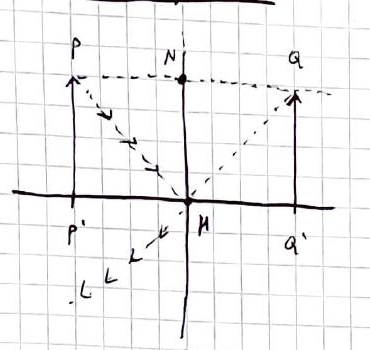
\includegraphics[width=.48\linewidth]{ottica_tex_assets/b36_p39_1.png}\end{center}
Nello specchio piano $R\to\infty$ ($C\to\infty$):
\[
\frac1p-\frac1q=-\frac2R\longrightarrow0
\quad\Longrightarrow\quad p=q,
\qquad I=\frac{y'}y=-\frac qp=-1.
\]
L'immagine non viene ingrandita/rimpicciolita e $I<0$, quindi rimane dritta.
\subsubsection*{Diottro}
Costituito da due mezzi trasparenti con indici di rifrazione diversi, $n_1<n_2$.
\begin{center}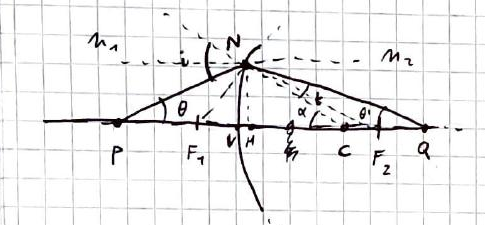
\includegraphics[width=.6\linewidth]{ottica_tex_assets/b36_p39_2.png}\end{center}
\[
i=\theta+\alpha,\qquad\alpha=\theta'+t,
\qquad n_1i=n_2t,\qquad n_1\sin i=n_2\sin t.
\]
\[
n_1(\alpha+\theta)=n_2(\alpha-\theta')
\quad\Longrightarrow\quad
\frac{n_1}{p}+\frac{n_2}{q}=\frac{n_2-n_1}{R}.
\]
Convesso:
\begin{center}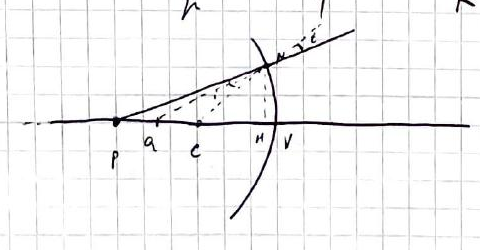
\includegraphics[width=.6\linewidth]{ottica_tex_assets/b36_p39_3.png}\end{center}
\[
\frac{n_1}{p}-\frac{n_2}{q}=-\frac{n_2-n_1}{R}.
\]
\subsubsection*{Convenzione dei segni}
\begin{center}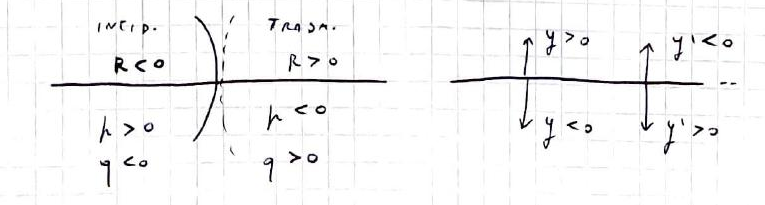
\includegraphics[width=.95\linewidth]{ottica_tex_assets/b36_p39_4.png}\end{center}
Lato incidente: $R<0$, $p>0$, $q<0$; lato trasmesso: $R>0$, $p<0$, $q>0$.
$y>0$ sopra l'asse, $y<0$ sotto; $y'<0$ sopra l'asse, $y'>0$ sotto.
% Pagina originale 40
\pagina{40}
\[
\frac{n_1}{p}+\frac{n_2}{q}=\frac{n_2-n_1}{R}.
\]
Equazione generale: convenzione dei segni.
\subsubsection*{Fuoco}
\[
P\to\infty\quad\Longrightarrow\quad p\to\infty,
\qquad
\frac{n_2}{q}=\frac{n_2-n_1}{R}
\quad\Longrightarrow\quad
q=f_2=\frac{n_2}{n_2-n_1}R.
\]
$f_2$: fuoco posteriore.
\[
Q\to\infty\quad\Longrightarrow\quad q\to\infty,
\qquad
\frac{n_1}{p}=\frac{n_2-n_1}{R}
\quad\Longrightarrow\quad
p=f_1=\frac{n_1}{n_2-n_1}R.
\]
$f_1$: fuoco anteriore.
\begin{center}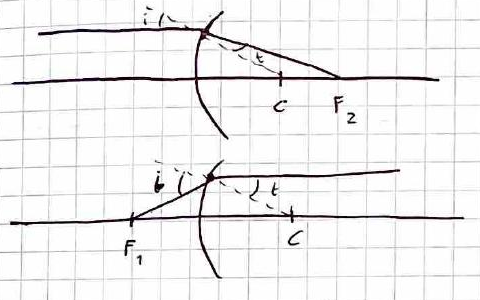
\includegraphics[width=.62\linewidth]{ottica_tex_assets/b36_p40_1.png}\end{center}
Primo caso: $p\to\infty$; secondo caso: $q\to\infty$.
\subsubsection*{Costruzione dell'immagine}
\begin{center}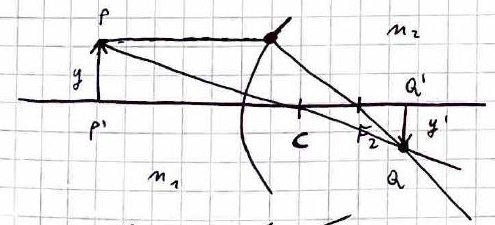
\includegraphics[width=.65\linewidth]{ottica_tex_assets/b36_p40_2.png}\end{center}
\[
I=\frac{y'}y\geq0\quad\Longrightarrow\quad\text{capovolta}
\qquad(y>0,\ y'\geq0).
\]
\begin{center}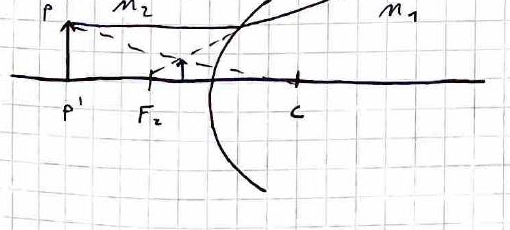
\includegraphics[width=.65\linewidth]{ottica_tex_assets/b36_p40_3.png}\end{center}
\[
I<0\qquad(y>0,\ y'<0),\qquad
I=\frac{n_1q}{n_2p}.
\]
% Pagina originale 41
\pagina{41}
\subsubsection*{Diottro piano}
\begin{center}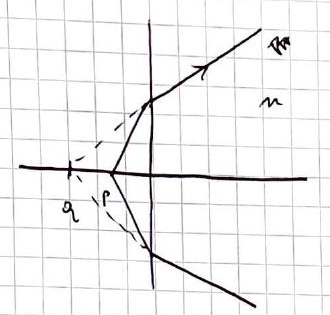
\includegraphics[width=.45\linewidth]{ottica_tex_assets/b36_p41_1.png}\end{center}
\[
\frac{n_1}{p}+\frac{n_2}{q}=\frac{n_2-n_1}{R},
\qquad R\to\infty\quad\Longrightarrow\quad
\frac{n_1}{p}=-\frac{n_2}{q}
\quad\Longrightarrow\quad q=-\frac{n_2}{n_1}p.
\]
\[
I=\frac{n_1q}{n_2p}
=\frac{n_1\left(-\frac{n_2}{n_1}p\right)}{n_2p}=-1<0.
\]
\subsubsection*{Lenti}
È l'insieme di due diottri.
\begin{center}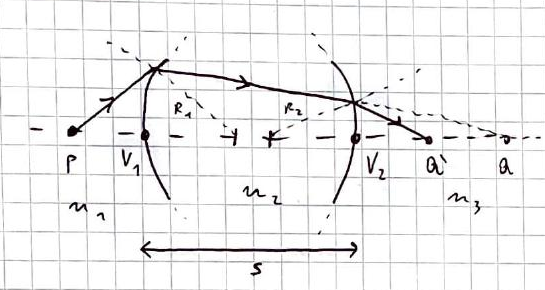
\includegraphics[width=.75\linewidth]{ottica_tex_assets/b36_p41_2.png}\end{center}
\[
\frac{n_1}{p_1}+\frac{n_2}{q_1}=\frac{n_2-n_1}{R_1},\qquad
\frac{n_2}{p_2}+\frac{n_3}{q_2}=\frac{n_3-n_2}{R_2},\qquad p_2=s-q_1.
\]
\[
n_1=n_3\quad\Longrightarrow\quad
\frac{n_1}{p_1}+\frac{n_2s}{q_1(s-q_1)}+\frac{n_1}{q_2}
=(n_2-n_1)\left(\frac1{R_1}-\frac1{R_2}\right).
\]
\subsubsection*{Lenti sottili}
\begin{center}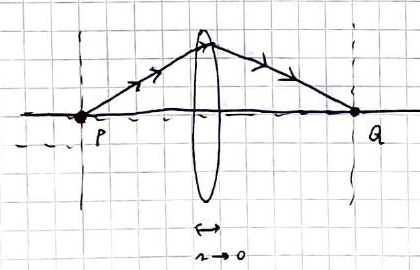
\includegraphics[width=.58\linewidth]{ottica_tex_assets/b36_p41_3.png}\end{center}
\[
s\to0,\qquad
\frac{n_1}{p_1}+\frac{n_1}{q_2}
=(n_2-n_1)\left(\frac1{R_1}-\frac1{R_2}\right),
\qquad p_1=p,\quad q_1=q.
\]
% Nella riga manoscritta prima dell'ultima formula l'indice di q appare 1; la formula precedente usa q_2. Si conserva q_1 nell'annotazione originale:

\[
\frac1p+\frac1q=\frac{n_2-n_1}{n_1}
\left(\frac1{R_1}-\frac1{R_2}\right)=\frac1f.
\]
% Pagina originale 42
\pagina{42}
\subsubsection*{Classificazione delle lenti}
\begin{center}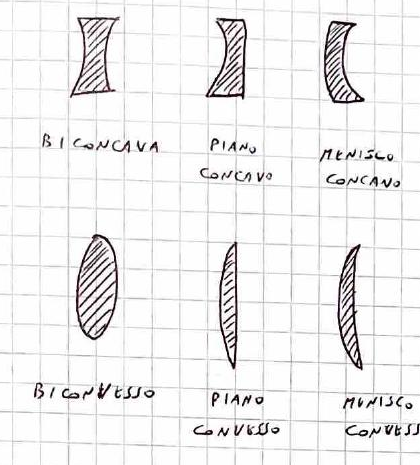
\includegraphics[width=.7\linewidth]{ottica_tex_assets/b36_p42_1.png}\end{center}
Divergenti: biconcava, piano-concava, menisco concavo; $1/f<0$.
Convergenti: biconvessa, piano-convessa, menisco convesso; $1/f>0$.
\subsubsection*{Lente convergente}
\begin{center}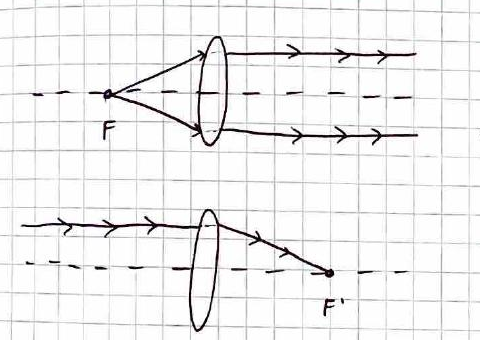
\includegraphics[width=.7\linewidth]{ottica_tex_assets/b36_p42_2.png}\end{center}
\[
q\to\infty\quad\Longrightarrow\quad p=f,
\qquad q\to\infty\quad\Longrightarrow\quad p=f,
\qquad p\to\infty\quad\Longrightarrow\quad q=f,
\qquad\frac1p+\frac1q=\frac1f.
\]
% La prima relazione q -> infinito è ripetuta due volte nella pagina originale.
\subsubsection*{Lente divergente}
\begin{center}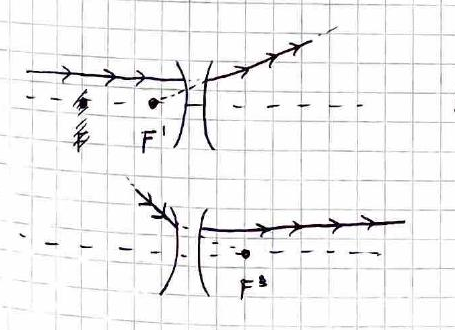
\includegraphics[width=.7\linewidth]{ottica_tex_assets/b36_p42_3.png}\end{center}
\[
p\to\infty\quad\Longrightarrow\quad q=f,
\qquad q\to\infty\quad\Longrightarrow\quad p=f.
\]
La distanza focale è sempre uguale:
\[
\frac1f=\frac1{f'}.
\]
% Pagina originale 43
\pagina{43}
\[
\frac1f=P\qquad\text{potenza (potere diottrico)}.
\]
È l'inverso della distanza focale. Unità di misura: $D$, diottrie,
\[
D=\frac1{\mathrm m}=\mathrm m^{-1}.
\]
$P>0$ per lenti convergenti; $P<0$ per lenti divergenti.
\subsubsection*{Costruzione dell'immagine}
\begin{center}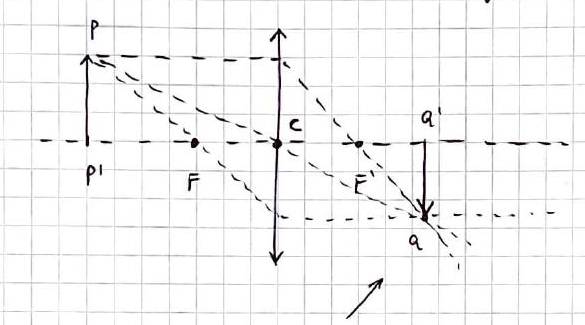
\includegraphics[width=.8\linewidth]{ottica_tex_assets/b36_p43_1.png}\end{center}
I raggi sono:
\begin{enumerate}
\item $P\to F'$;
\item $P\to F$: parallelo;
\item $P\to C$.
\end{enumerate}
Immagine reale e capovolta.
\begin{center}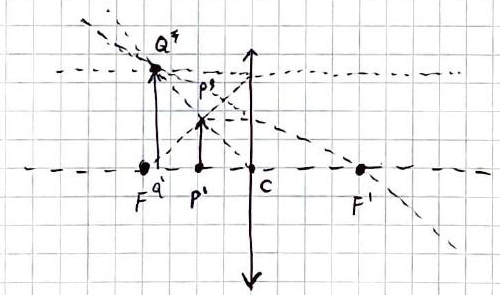
\includegraphics[width=.7\linewidth]{ottica_tex_assets/b36_p43_2.png}\end{center}
$P\in(F,C)$: immagine virtuale e dritta.
\begin{center}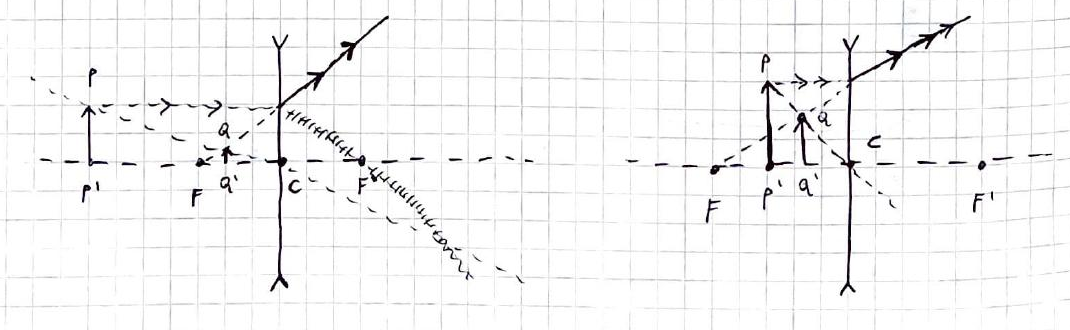
\includegraphics[width=\linewidth]{ottica_tex_assets/b36_p43_3.png}\end{center}
Nei due casi rappresentati: immagine virtuale e dritta.
% Pagina originale 44
\pagina{44}
\subsubsection*{Ingrandimento}
\[
I=\frac qp=\frac{q-f}{q}=\frac f{p-f}.
\]
% La frazione intermedia (q-f)/q è quella manoscritta, benché non coincida in generale con q/p.
\subsubsection*{Sistema di lenti}
\[
\text{Oggetto}_1\xrightarrow{\text{lente 1}}\text{Immagine}_1
=\text{Oggetto}_2\xrightarrow{\text{lente 2}}\text{Immagine}_2.
\]
Si può dimostrare che
\[
\frac1{f_{\mathrm{eq}}}=\frac1{f_1}+\frac1{f_2},\qquad
P_{\mathrm{eq}}=\sum_i P_i.
\]
Le lenti si dicono \emph{addossate} se la loro distanza è nulla o trascurabile.
\begin{center}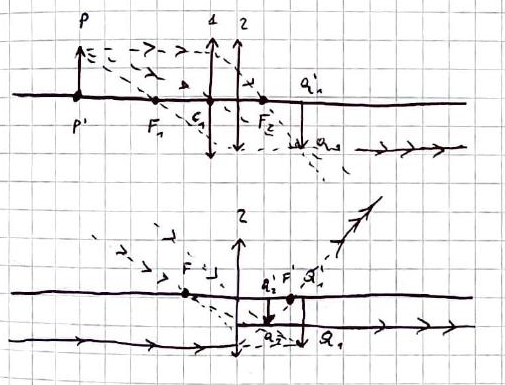
\includegraphics[width=.7\linewidth]{ottica_tex_assets/b36_p44_1.png}\end{center}
$Q_1$ è un'immagine virtuale che diventa oggetto virtuale per la lente 2. $Q_2$ è l'immagine finale.
\begin{align*}
\frac1{p_1}+\frac1{q_1}&=\frac1{f_1},\\
\frac1{p_2}+\frac1{q_2}&=-\frac1{q_1}+\frac1{q_2}=\frac1{f_2}.
\end{align*}
\[
\begin{cases}\frac1p+\frac1{q_1}=\frac1{f_1},\\
\frac1q-\frac1{q_1}=\frac1{f_2},\end{cases}
\quad\Longrightarrow\quad
\frac1p+\frac1q=\frac1{f_1}+\frac1{f_2}
\quad\Longrightarrow\quad
\frac1f=\frac1{f_1}+\frac1{f_2}.
\]
% Pagina originale 45
\pagina{45}
\subsubsection*{Occhio}
\begin{itemize}
\item Coroide: assorbe la luce dispersa.
\item Cornea: devia gran parte della luce.
\item Umor acqueo: liquido tra cornea e cristallino (indice $n$: valore tagliato al margine destro, pagina 45).
\item Pupilla: determina la quantità di luce che entra nell'occhio.
\item Cristallino: lente biconvessa con $n\simeq1{,}47$.
\item Umor vitreo: sostanza gelatinosa tra cristallino e retina ($n\simeq1{,}33$).
\end{itemize}
Potere diottrico:
\[
P_0=60\,D\quad\Longrightarrow\quad f=\frac1D=17\,\mathrm{mm}.
\]
\subsubsection*{Immagini reali e virtuali}
\paragraph{Specchi}
\[
\frac1p-\frac1q=-\frac2R.
\]
\begin{itemize}
\item Piani: sempre virtuale, dritta, $I=-1$.
\item Concavi: reale se $p>f$, immagine capovolta; virtuale se $p<f$, immagine dritta.
\item Convessi: sempre virtuale, dritta, $|I|<1$.
\end{itemize}
Negli specchi è reale se lo specchio è concavo e $p>f$.
\paragraph{Lenti}
\[
\frac1p+\frac1q=\frac1f.
\]
\begin{itemize}
\item Convergenti: reale se $p>f\Rightarrow q>0$; virtuale se $p<f\Rightarrow q<0$.
\item Divergenti: sempre virtuale ($q<0$), dritta, $|I|<1$.
\end{itemize}
\paragraph{Diottri}
\[
\frac{n_1}{p}+\frac{n_2}{q}=\frac{n_2-n_1}{R},\qquad
q<0\ \longrightarrow\ \text{virtuale},\qquad
q>0\ \longrightarrow\ \text{reale}.
\]
% Pagina originale 46
\pagina{46}
\subsubsection*{Interferenza}
\begin{center}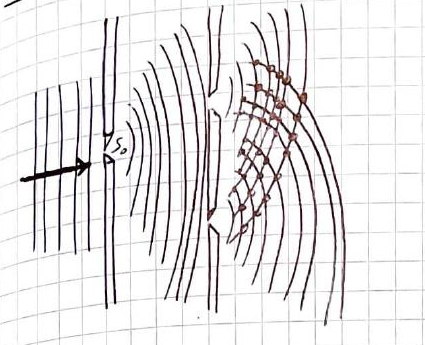
\includegraphics[width=.55\linewidth]{ottica_tex_assets/b36_p46_1.png}\end{center}
\begin{align*}
\vv E_1(r,t)&=\frac{\vv E_0}{r}\sin(kr-\omega t+\phi_1),\\
\vv E_2(r,t)&=\frac{\vv E_0}{r}\sin(kr-\omega t+\phi_2),\\
\delta&=k(r_2-r_1)+(\phi_2-\phi_1)\qquad\text{differenza di fase}.
\end{align*}
Se $\Delta\phi=0$, allora $\delta=k(r_2-r_1)$.
\begin{center}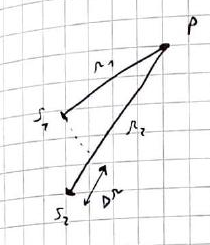
\includegraphics[width=.3\linewidth]{ottica_tex_assets/b36_p46_2.png}\end{center}
Se $\partial\delta/\partial t=0$ (costante nel tempo) le sorgenti si dicono coerenti.
\[
\frac{\partial\delta}{\partial t}\ne0\quad\Longrightarrow\quad\text{sorgenti incoerenti}.
\]
\subsubsection*{Esperimento di Young}
\begin{center}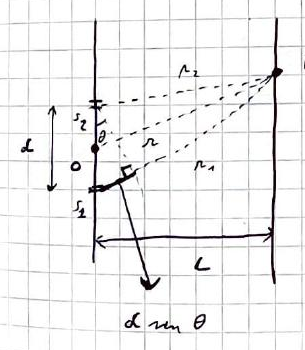
\includegraphics[width=.43\linewidth]{ottica_tex_assets/b36_p46_3.png}\end{center}
Prendiamo due onde sferiche con stessa lunghezza d'onda (quindi stesso $k$):
\[
\vv E_1(r,t)=\frac{\vv E_0}{r}\sin(kr-\omega t),\qquad
\vv E_2(r,t)=\frac{\vv E_0}{r}\sin(kr-\omega t).
\]
\begin{align*}
\vv E_P&=\vv E_1(r,t')+\vv E_2(r,t')\\
&=\frac{\vv E_0}{r_1}\sin(kr_1-\omega t')+
\frac{\vv E_0}{r_2}\sin(kr_2-\omega t').
\end{align*}
Poniamo $r\simeq r_1\simeq r_2$:
\[
\vv E_P=\frac{\vv E_0}{r}\left[
\sin\left(\frac{kr_1-\omega t'+kr_2-\omega t'}2\right)
\cos\left(\frac{kr_1-\omega t'-kr_2+\omega t'}2\right)
\right].
\]
% La formula manoscritta non mostra il fattore 2 della somma di seni; conservata.
% Pagina originale 47
\pagina{47}
Sfruttando la formula di sovrapposizione:
\begin{align*}
A\left[\sin(k_1x-\omega_1t)+\sin(k_2x-\omega_2t)\right]
&=2A\cos\left(\frac{\Delta k}{2}x-\frac{\Delta\omega}{2}t\right)
\sin(k_mx-\omega_mt),
\end{align*}
$k_m$, $\omega_m$: medie. Quindi
\[
\vv E_P=2\frac{\vv E_0}{r}
\sin\left(\frac{k(r_1+r_2)}2-\omega t'\right)
\cos\left(\frac{k(r_1-r_2)}2\right).
\]
\[
\frac{r_1+r_2}{2}\simeq r,\qquad\delta=k(r_1-r_2),
\]
\[
\vv E_P=2\frac{\vv E_0}{r}\sin(kr-\omega t')\cos\frac\delta2,
\quad\text{cioè}\quad
\vv E_P=2\frac{\vv E_0}{r}\cos\frac\delta2\cdot\sin(kr-\omega t'),
\qquad |\vv E_P|=2\frac{E_0}{r}\cos\frac\delta2.
\]
\begin{align*}
I&=c\varepsilon_0\langle E_P^2\rangle
=c\varepsilon_0\left[2\frac{E_0}{r}\cos\frac\delta2\right]^2
\langle\sin^2(kr-\omega t')\rangle\\
&=\frac12\,4\frac{E_0^2}{r^2}\cos^2\frac\delta2\,c\varepsilon_0
=4\frac{I_0}{r^2}\cos^2\frac\delta2
\qquad(I\propto\delta).
\end{align*}
\[
\delta=k(r_1-r_2)=\frac{2\pi}{\lambda}(r_1-r_2),\qquad
r_1-r_2\simeq d\sin\theta.
\]
\begin{align*}
I&=4\frac{I_0}{r^2}\cos^2\frac\delta2\simeq4I_0\cos^2\frac\delta2\\
&=4I_0\cos^2\left(\frac{kd\sin\theta}2\right)
=4I_0\cos^2\left(\frac{\pi d\sin\theta}{\lambda}\right).
\end{align*}
\[
I_{\max}=4I_0\quad\Longrightarrow\quad
\frac{\pi d\sin\theta}{\lambda}=m\pi,
\qquad
I_{\min}=0\quad\Longrightarrow\quad
\frac{\pi d\sin\theta}{\lambda}=\left(m+\frac12\right)\pi.
\]
% Si conserva il passaggio approssimato che assorbe 1/r^2 in I_0 e l'annotazione I proporzionale a delta dell'originale.
% Pagina originale 48
\pagina{48}
Cioè
\[
d\sin\theta=m\lambda\quad\text{massimi},\qquad
d\sin\theta=\left(m+\frac12\right)\lambda\quad\text{minimi}.
\]
Se $L\gg d$:
\[
\sin\theta\simeq\tan\theta\simeq\theta=\frac xL,
\qquad I(x)=4I_0\cos^2\left(\frac{\pi d}{\lambda L}x\right).
\]
Quindi
\begin{align*}
x_M&=\frac Ld m\lambda
\quad\Longrightarrow\quad
\theta_M=\frac{x_M}{L}=\frac Ld m\lambda\cdot\frac1L,\\
x_m&=\frac Ld\left(m+\frac12\right)\lambda
\quad\Longrightarrow\quad
\theta_m=\frac{x_m}{L}=\frac{L\lambda}{d}\left(m+\frac12\right)\frac1L.
\end{align*}
\[
\theta_M=\frac\lambda d m,\qquad
\theta_m=\frac\lambda d\left(m+\frac12\right).
\]
\begin{center}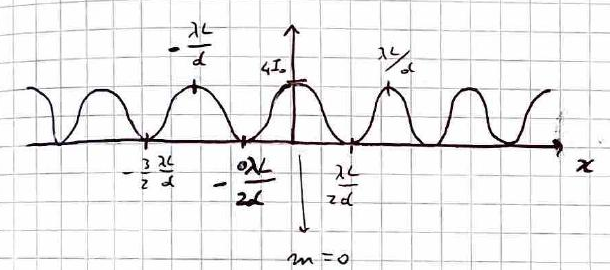
\includegraphics[width=.82\linewidth]{ottica_tex_assets/b36_p48_1.png}\end{center}
I passi
\[
p_M=x_{M+1}-x_M=\frac{\lambda L}{d}
\]
sono le distanze tra due frange chiare (massimi).
Se le onde si propagano in un mezzo con indice di rifrazione $n$:
\[
\delta=kn(r_1-r_2)=\frac{2\pi}{\lambda}nd\sin\theta,
\]
\[
I(\theta)=4I_0\cos^2\left(n\frac{\pi d\sin\theta}{\lambda}\right),\qquad
I(x)=4I_0\cos^2\left(n\frac{\pi dx}{\lambda L}\right).
\]
% Pagina originale 49
\pagina{49}
\subsubsection*{Sorgenti incoerenti}
\[
\delta=k(r_2-r_2)+(\phi_2-\phi_1)
=k(r_2-r_1)+\Delta\phi(t).
\]
% Il primo termine manoscritto sembra r_2-r_2, mentre nella stessa riga è poi r_2-r_1; refuso conservato.
\[
\vv E_P=\left[2\frac{\vv E_0}{r}\cos\left(\frac{\delta+\Delta\phi(t)}2\right)\right]
\sin(kr-\omega t').
\]
\begin{align*}
I&=c\varepsilon_0\langle E_P^2\rangle
=c\varepsilon_0\left[2\frac{E_0}{r}\right]^2
\left\langle\cos^2\left(\frac{\delta+\Delta\phi(t)}2\right)\right\rangle
\langle\sin^2(kr-\omega t')\rangle\\
&=c\varepsilon_0\,4\frac{E_0^2}{r^2}\cdot\frac12\cdot\frac12
=2\frac{I_0}{r^2}.
\end{align*}
\[
I=2I_0\frac1{r^2}\qquad\text{costante e non dipendente da }x.
\]
\subsubsection*{Effetto cromatico}
\[
I(\theta)=4I_0\cos^2\left(\frac{\pi d\sin\theta}{\lambda}\right)
\propto\cos^2\frac{\cdots}{\lambda}.
\]
Dipende da $\lambda$.
\[
x(\lambda)=m\frac{\lambda L}{d}
\]
Cambia per ogni colore: $x_{m=1,\mathrm{rosso}}\ne x_{m=1,\mathrm{blu}}$, ecc.
\begin{center}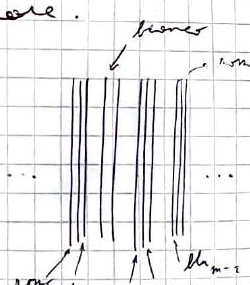
\includegraphics[width=.38\linewidth]{ottica_tex_assets/b36_p49_1.png}\end{center}
\subsubsection*{Lamine sottili}
\begin{center}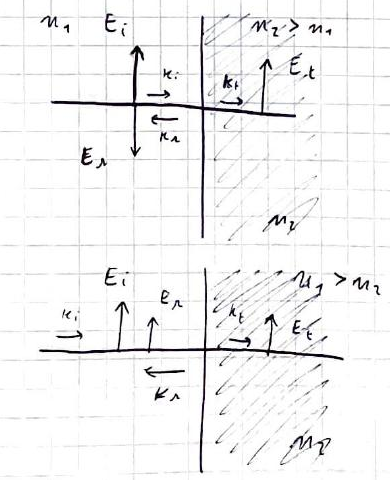
\includegraphics[width=.52\linewidth]{ottica_tex_assets/b36_p49_2.png}\end{center}
Se $n_2>n_1$: $r_0<0$ (sfasato di $\pi$), $t_0>0$ (in fase).
Se $n_1>n_2$: $r_0>0$, $t_0>0$ (in fase).
% Pagina originale 50
\pagina{50}
\begin{center}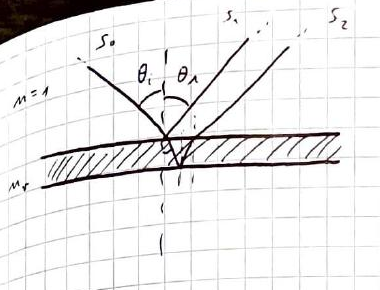
\includegraphics[width=.55\linewidth]{ottica_tex_assets/b36_p50_1.png}\end{center}
\[
\delta=k(r_1-r_2)+\Delta\phi(t),\qquad
\phi_1=\phi_0+\pi\quad(n>1),\qquad\phi_2=\phi_0.
\]
\[
\phi_2-\phi_1=\phi_0-(\phi_0+\pi)=-\pi=\Delta\phi.
\]
\begin{align*}
\delta&=k(r_2-r_1)+\Delta\phi=k(2nd\cos\theta_r)-\pi\\
&=2kd\sqrt{n^2-\sin^2\theta_i}-\pi.
\end{align*}
Quando c'è incidenza normale, $\theta_i=\theta_r=0$:
\[
\delta=2kdn-\pi=\frac{4\pi dn}{\lambda}-\pi.
\]
\begin{align*}
I&=4I_0\cos^2\frac\delta2
=4I_0\cos^2\left(\frac{4\pi dn}{\lambda}-\pi\right)\\
&=4I_0\left[-\cos\left(\frac{4\pi dn}{\lambda}\right)\right]^2
=4I_0\cos^2\left(\frac{2\pi dn}{\lambda}\right).
\end{align*}
% I passaggi intermedi del manoscritto omettono la divisione per 2 dell'argomento; conservati senza correzioni silenziose.
\[
\frac\delta2=m\pi\qquad\text{interferenza costruttiva},\qquad
\frac\delta2=\left(m+\frac12\right)\pi\qquad\text{interferenza distruttiva}.
\]
\[
d=\left(m+\frac12\right)\frac\lambda{2n}\quad\text{I.C.},\qquad
d=m'\frac\lambda{2n}\quad\text{I.D.}
\]
\subsubsection*{Cuneo sottile}
\begin{center}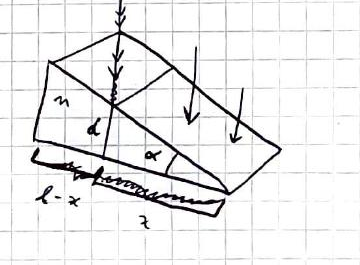
\includegraphics[width=.55\linewidth]{ottica_tex_assets/b36_p50_2.png}\end{center}
Se $\alpha\simeq0$, allora
\[
\tan\alpha\simeq\alpha=\frac dx.
\]
Trattiamo il cuneo come una lamina sottile.
% Pagina originale 51
\pagina{51}
\[
d=\left(m+\frac12\right)\frac\lambda{2n}
\quad\Longrightarrow\quad
\alpha=\left(m+\frac12\right)\frac\lambda{2nx}
\quad\Longrightarrow\quad
x=\left(m+\frac12\right)\frac\lambda{2n\alpha}\quad\text{I.C.}
\]
\[
x=m'\frac\lambda{2n\alpha}\qquad\text{I.D.}
\]
\subsubsection*{Anelli di Newton}
\begin{center}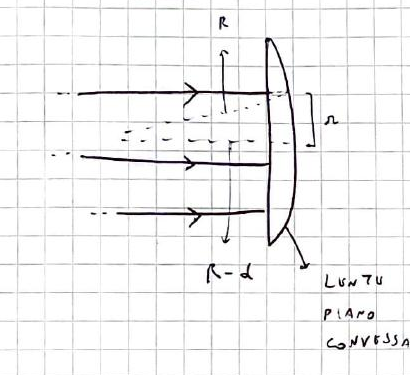
\includegraphics[width=.5\linewidth]{ottica_tex_assets/b36_p51_1.png}\end{center}
Lente piano-convessa:
\begin{align*}
r^2&=R^2-(R-d)^2=-d^2+2Rd,\\
\frac{r^2}{4R^2}&=\frac d{2R}-\left(\frac d{2R}\right)^2,\\
d\ll R&\quad\Longrightarrow\quad\frac{r^2}{4R^2}=\frac d{2R}
\quad\Longrightarrow\quad r^2=2Rd.
\end{align*}
Il sistema è simile al cuneo.
\[
d=\left(m+\frac12\right)\frac\lambda{2n}
\quad\Longrightarrow\quad
r^2=\left(m+\frac12\right)\frac{2R\lambda}{2n}.
\]
\[
r=\sqrt{\left(m+\frac12\right)R\lambda}\quad\text{I.C.},\qquad
r=\sqrt{m'R\lambda}\quad\text{I.D.}
\]
% Le ultime espressioni originali non riportano il fattore 1/n.
\subsubsection*{Interferenza di $N$ sorgenti}
\begin{center}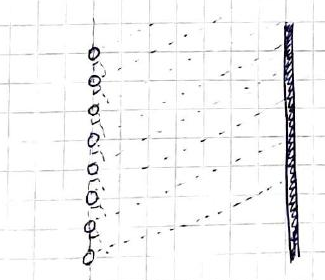
\includegraphics[width=.42\linewidth]{ottica_tex_assets/b36_p51_2.png}\end{center}
\[
\delta=k(r_i-r_{i+1})=\frac{2\pi}{\lambda}(r_i-r_{i+1}),
\qquad
\vv E_0=\vv E_0\sin(kx-\omega t),\qquad
\vv E_i=\vv E_0\sin(kx-\omega t+i\delta).
\]
% Pagina originale 52
\pagina{52}
\begin{align*}
\vv E_P(r,t)&=\vv E_1(r,t)+\vv E_2(r,t)+\cdots+\vv E_N(r,t),\\
\vv E_P(r,t)&=\sum_{i=1}^{N}\vv E_i(r,t)
=\vv E_0\sum_{i=1}^{N}\sin(kr-\omega t+i\delta).
\end{align*}
Trattiamo i moduli:
\[
E_0=2\rho\sin\frac\delta2,\qquad E_P=2\rho\sin\frac{N\delta}{2}.
\]
\[
E_P=E_0\frac{\sin(N\delta/2)}{\sin(\delta/2)}
\quad\Longrightarrow\quad
I_P=I_0\frac{\sin^2(N\delta/2)}{\sin^2(\delta/2)}.
\]
Calcoliamo $\delta$:
\[
\delta=k(r_i-r_{i+1})=\frac{2\pi}{\lambda}d\sin\theta.
\]
\[
I_P(\theta)=I_0\frac{\sin^2(N\delta/2)}{\sin^2(\delta/2)}
=I_0\left[\frac{\sin(\pi Nd\sin\theta/\lambda)}
{\sin(\pi d\sin\theta/\lambda)}\right]^2.
\]
Se $N=2$:
\[
I_P(\theta)=I_0\frac{\left(2\sin\frac\delta2\cos\frac\delta2\right)^2}
{\left(\sin\frac\delta2\right)^2}=4I_0\cos^2\frac\delta2.
\]
\begin{center}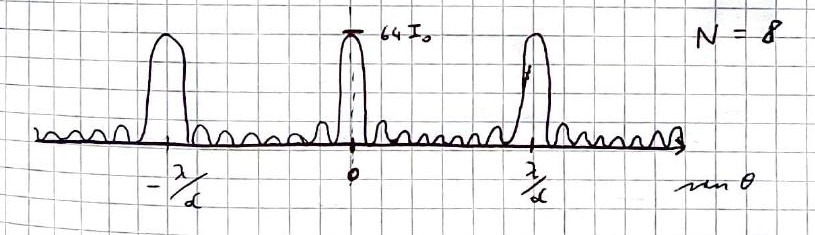
\includegraphics[width=\linewidth]{ottica_tex_assets/b36_p52_1.png}\end{center}
$N=8$, massimo centrale $64I_0$; ascissa $\sin\theta$, massimi a $-\lambda/d$, $0$, $\lambda/d$.
\[
\lim_{\delta\to0}I_0\frac{\sin^2(N\delta/2)}{\sin^2(\delta/2)}
=\lim_{\delta\to0}I_0\frac{N^2\delta^2/4}{\delta^2/4}=I_0N^2.
\]
$I_{\max}$: massimi principali.
I massimi principali si hanno quando il denominatore tende a zero:
\[
\Delta(\sin\theta)_{\max}=\frac\lambda d,
\]
\[
I_M=\lim_{\frac\pi\lambda d\sin\theta\to m\pi}
I_0\frac{\sin^2(N\pi d\sin\theta/\lambda)}
{\sin^2(\pi d\sin\theta/\lambda)}=N^2I_0.
\]
% Pagina originale 53
\pagina{53}
Il minimo si ha quando il numeratore tende a zero (e il denominatore non è diverso da zero, come scritto negli appunti).
% L'inciso originale «den. non è diverso da 0» è conservato, pur essendo incoerente con la condizione sui minimi.
\[
\sin^2\left(\frac{N\pi}{\lambda}d\sin\theta\right)\to0
\quad\Longrightarrow\quad\frac{N\pi}{\lambda}d\sin\theta\to0,
\]
\[
\sin\theta\,\frac{N\pi}{\lambda}d=m'\pi
\quad\Longrightarrow\quad\sin\theta=\frac{m'\lambda}{Nd}.
\]
\[
(\sin\theta)_{\min}=(\sin\theta)_{\max}
\quad\Longleftrightarrow\quad m'\frac\lambda{Nd}=m\frac\lambda d
\quad\Longrightarrow\quad m'=Nm.
\]
$m'$ non è un minimo ma un massimo.
I massimi secondari si hanno quando il seno è 1:
\[
\sin^2\left(\frac{N\pi}{\lambda}d\sin\theta\right)=1
\quad\Longrightarrow\quad
\frac{N\pi}{\lambda}d\sin\theta=\left(m''+\frac12\right)\pi\lambda,
\]
% L'ultima lambda della riga manoscritta è conservata; il passaggio seguente non la include.
\[
\sin\theta=\left(m''+\frac12\right)\frac\lambda{Nd},
\qquad m''=0,\pm1,\pm2,\ldots
\]
\[
I''=\frac{I_0}{\sin^2\left((m''+\frac12)\frac\pi N\right)}
=\frac{I_M}{N^2\sin^2\left((m''+\frac12)\frac\pi N\right)}.
\]
\[
(\sin\theta)_{m'=1}=\frac\lambda{Nd},\qquad
(\sin\theta)_{m'=-1}=-\frac\lambda{Nd},\qquad
\Delta(\sin\theta)=\frac{2\lambda}{Nd}.
\]
Larghezza angolare dei massimi principali:
\begin{center}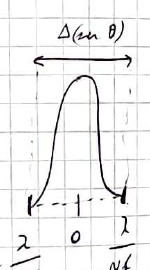
\includegraphics[width=.3\linewidth]{ottica_tex_assets/b36_p53_1.png}\end{center}
\subsubsection*{Caratteristiche}
\begin{itemize}
\item $m=0$: massimo principale.
\item Tra due massimi principali ci sono $N-2$ massimi secondari.
\item Tra due massimi principali ci sono $N-1$ minimi.
\item $I_{\max,\mathrm{pr}}=N^2I_0$.
\item Ampiezza angolare $\propto1/N$.
\item $I_{\max,\mathrm{sec}}\propto\frac1{N^2}I_{\max,\mathrm{pr}}$
($I_{\max,\mathrm{sec}}\simeq I_0$).
\end{itemize}
% Pagina originale 54
\pagina{54}
\begin{center}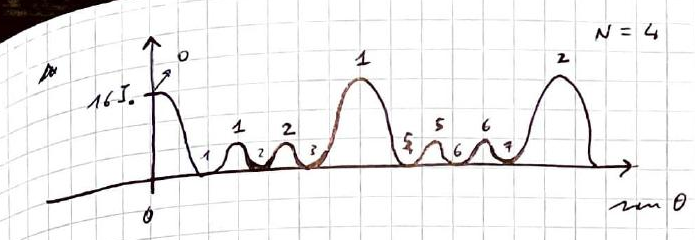
\includegraphics[width=.85\linewidth]{ottica_tex_assets/b36_p54_1.png}\end{center}
$N=4$:
\[
\text{max P}:\ \sin\theta=m\frac\lambda d,\qquad
\text{max S}:\ \sin\theta=\left(m''+\frac12\right)\frac\lambda{Nd},\qquad
\text{min}:\ \sin\theta=m'\frac\lambda{Nd}.
\]
\begin{center}\small
\begin{tabular}{c|*{11}{c}}
$\frac d\lambda\sin\theta$&0&$\frac18$&$\frac28$&$\frac38$&$\frac12$&$\frac58$&$\frac34$&$\frac78$&1&$\frac98$&$\frac54$\\\hline
$m$, max P&0&&&&&&&&1&&\\
$m''$, max S&&0&&1&&2&&3&&4&\\
$m'$, min&0&&1&&2&&3&&4&&5
\end{tabular}
\end{center}
$m'=0$ e $m'=4$ per i minimi non sono valori validi perché $m'=Nm$ ($m'$ multiplo di $N$).
$m''=0$, $m''=3$, $m''=4$ non sono validi perché compresi tra il massimo principale ed il primo minimo (o tra l'ultimo minimo e il massimo principale).
\subsubsection*{Diffrazione}
La diffrazione è una particolare interferenza che avviene quando le dimensioni dell'ostacolo sono prossime alla lunghezza d'onda della radiazione.
Esistono due tipi di diffrazione:
\begin{itemize}
\item Fresnel: campo vicino;
\item Fraunhofer: campo lontano.
\end{itemize}
% Pagina originale 55
\pagina{55}
\subsubsection*{Diffrazione di Fraunhofer: fenditura singola}
\begin{center}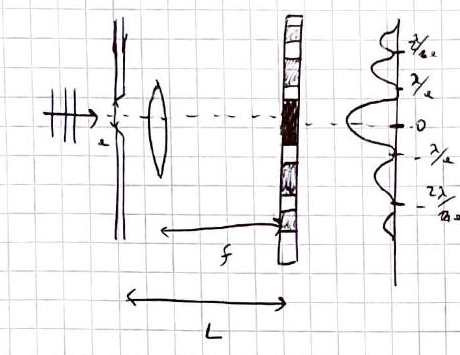
\includegraphics[width=.62\linewidth]{ottica_tex_assets/b36_p55_1.png}\end{center}
Divido la fenditura in $N$ sorgenti:
\[
\Delta y=\frac aN,\qquad
\Delta\phi=\frac{2\pi}{\lambda}\Delta y\sin\theta
\quad[=k(y_i-y_{i+1})].
\]
\[
\alpha=\frac{2\pi}{\lambda}a\sin\theta
\qquad\text{è la differenza di fase totale}.
\]
\[
\begin{cases}E_P=2\rho\sin\frac\alpha2,\\E_{\max}=\rho\alpha,\end{cases}
\quad\Longrightarrow\quad E_P=2\frac{E_{\max}}\alpha\sin\frac\alpha2.
\]
\[
E_P(\theta)=E_{\max}\frac{\sin(\alpha/2)}{\alpha/2}
=E_{\max}\frac{\sin(\frac\pi\lambda a\sin\theta)}
{\frac\pi\lambda a\sin\theta}.
\]
\[
I_P(\theta)=I_{\max}\left(\frac{\sin(\frac\pi\lambda a\sin\theta)}
{\frac\pi\lambda a\sin\theta}\right)^2.
\]
\[
I_P=I_{\max}\quad\text{se}\quad\frac\pi\lambda a\sin\theta\to0.
\]
Questa condizione si realizza solo quando $\theta=0$ e si parla di massimo centrale.
I minimi si hanno quando si annulla il numeratore:
\[
\frac\pi\lambda a\sin\theta=m\pi
\quad\Longrightarrow\quad\sin\theta=m\frac\lambda a,
\qquad m=\pm1,\pm2,\ldots
\]
I massimi secondari si hanno quando il seno è 1:
\[
\frac\pi\lambda a\sin\theta=\left(m'+\frac12\right)\pi
\quad\Longrightarrow\quad
\sin\theta=\left(m'+\frac12\right)\frac\lambda a,\qquad m'=1,2,\ldots
\]
% Pagina originale 56
\pagina{56}
\[
\frac{I_P}{I_{\max}}=\frac1{\pi^2(m'+\frac12)^2}.
\]
Con $m'=1$: $I_{\mathrm{sec},P}=0{,}045I_{\max}$.
La maggior parte della potenza si trova nella frangia centrale ($\simeq80\%$).
\[
\Delta(\sin\theta)=2\frac\lambda a
\quad\Longrightarrow\quad
\Delta\theta=2\frac\lambda{a\cos\theta}
\xrightarrow{\theta\simeq0}\Delta\theta=2\frac\lambda a.
\]
\subsubsection*{Diffrazione da apertura circolare}
Primo minimo di intensità:
\[
\sin\theta=1{,}22\frac\lambda D,
\qquad D:\ \text{diametro}.
\]
La larghezza angolare del massimo è $2\theta=\phi$.
\subsubsection*{Criterio di Rayleigh}
Due figure di diffrazione sono risolte se il massimo centrale di una cade nel primo zero dell'altra.
\subsubsection*{Interferenza e diffrazione: doppia fenditura sottile}
\begin{center}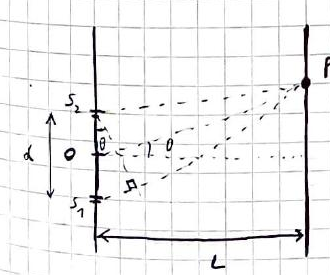
\includegraphics[width=.48\linewidth]{ottica_tex_assets/b36_p56_1.png}\end{center}
\[
E_{P1}(\theta)=E_0\frac{\sin(\frac\pi\lambda a\sin\theta)}
{\frac\pi\lambda a\sin\theta},\qquad
E_{P2}(\theta)=E_0\frac{\sin(\frac\pi\lambda a\sin\theta)}
{\frac\pi\lambda a\sin\theta}.
\]
Uso Carnot:
\begin{align*}
E_P^2&=E_{P1}^2+E_{P2}^2-2E_{P1}E_{P2}\cos(\pi-\delta)\\
&=E_{P1}^2+E_{P2}^2+2E_{P1}E_{P2}\cos\delta.
\end{align*}
% Pagina originale 57
\pagina{57}
Con $I=\frac12c\varepsilon_0 E^2$:
\[
I_P=2I_0\left[\frac{\sin(\frac\pi\lambda d\sin\theta)}
{\frac\pi\lambda a\sin\theta}\right]^2(1+\cos\delta)
=4I_0\left[\frac{\sin(\frac\pi\lambda a\sin\theta)}
{\frac\pi\lambda a\sin\theta}\right]^2\cos^2\frac\delta2.
\]
% Nel primo numeratore la lettera manoscritta è d; nella forma finale è a. Si conservano entrambe.
\[
\delta=\frac{2\pi d\sin\theta}{\lambda},\qquad
I_{\max}=N^2I_0.
\]
\[
I_P=I_{\max}
\underbrace{\left(\frac{\sin(\frac\pi\lambda a\sin\theta)}
{\frac\pi\lambda a\sin\theta}\right)^2}_{\text{fattore di diffrazione}}
\underbrace{\cos^2\left(\frac\pi\lambda d\sin\theta\right)}_{\text{fattore di interferenza}}.
\]
\paragraph{Esempio}
\begin{center}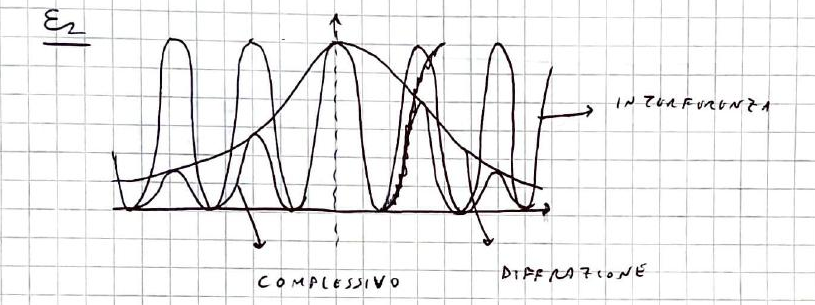
\includegraphics[width=\linewidth]{ottica_tex_assets/b36_p57_1.png}\end{center}
Massimi di interferenza:
\[
\sin\theta=m\frac\lambda d.
\]
Minimi di diffrazione:
\[
\sin\theta=m'\frac\lambda a.
\]
Possiamo dire che sono visibili solo i massimi di interferenza prima del primo minimo di diffrazione:
\[
\sin\theta=m\frac\lambda d<\frac\lambda a
\quad\Longrightarrow\quad m<\frac da.
\]
% Pagina originale 58
\pagina{58}
\subsubsection*{Nel caso di $N$ sorgenti}
\[
I_P=I_{\max}
\underbrace{\left(\frac{\sin(\frac\pi\lambda a\sin\theta)}
{\frac\pi\lambda a\sin\theta}\right)^2}_{\text{fattore di diffrazione}}
\underbrace{\left(\frac{\sin(\frac{\pi N}{\lambda}d\sin\theta)}
{\sin(\frac\pi\lambda d\sin\theta)}\right)^2}_{\text{fattore di interferenza}}.
\]
% La formula originale usa I_max senza il fattore di normalizzazione 1/N^2.
Anche qui $m<d/a$ è la condizione di visibilità.
% Pagina originale 59
\pagina{59}
\subsubsection*{Equazione di d'Alembert}
\[
\frac{\partial^2\xi}{\partial t^2}=v^2\frac{\partial^2\xi}{\partial x^2},\qquad
k=\frac{2\pi}{\lambda},\qquad\omega=2\pi f,\qquad
v=\frac\omega k,\qquad\lambda=\frac vf,\qquad
T=\frac1f,\qquad k=\frac\omega v.
\]
\subsubsection*{Onde sonore}
\[
v_s=\sqrt{\frac\beta\rho},\qquad
\mathrm{dB}=10\log_{10}\frac I{I_0}
=10(\log_{10}I+12),\qquad I_0=10^{12}.
\]
\subsubsection*{Sovrapposizione}
\[
\xi=2\xi_0\cos\left(\frac{\Delta k}{2}x-\frac{\Delta\omega}{2}t\right)
\sin(k_mx-\omega_mt).
\]
\subsubsection*{Effetto Doppler}
\[
f'=f\left(\frac{v_{\mathrm{onda}}\pm v_{\mathrm{oss}}}
{v_{\mathrm{onda}}\mp v_{\mathrm{sorg}}}\right).
\]
Segni superiori: avvicinamento; segni inferiori: allontanamento.
\[
kE=\omega B\quad\Longrightarrow\quad B=\frac Ec,
\qquad
\vv E\times\vv B=\frac{E^2}{c}\hat u_k=EB\hat u_k.
\]
\begin{center}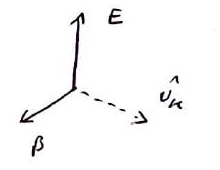
\includegraphics[width=.32\linewidth]{ottica_tex_assets/b36_p59_1.png}\end{center}
\[
n=\sqrt{\varepsilon_r\mu_r}\qquad\text{ma }\mu_r=1\text{ quasi sempre},
\qquad n=\frac cv\geq1.
\]
\[
\vv S=\frac{EB}{\mu_0}\hat u_k=\frac1{\mu_0}(\vv E\times\vv B)
\qquad\text{vettore di Poynting}.
\]
\[
p_{\mathrm{rad}}=\frac Ic(1+\eta)
\qquad\text{con }\eta\text{ coefficiente di riflessione}.
\]
\[
I=\frac P\Sigma,\qquad I=\frac12c\varepsilon_0E^2,\qquad
\varepsilon_0=8{,}85\cdot10^{-12}.
\]
% Nella pagina originale I_0 è annotato come 10^{12}, senza meno; conservato.
% Pagina originale 60
\pagina{60}
\[
P=\frac U{\Delta t}\quad\left(=\frac{\partial U}{\partial t}\right).
\]
\subsubsection*{Polarizzazione}
\[
I'=\underbrace{I\cos^2\theta}_{\text{legge di Malus}}
\quad\text{polarizzata},\qquad
I'=\frac I2\quad\text{non polarizzata}.
\]
\subsubsection*{Snell}
\[
n_1\sin\theta_1=n_2\sin\theta_2.
\]
\subsubsection*{Coefficienti di Fresnel}
\[
\chi=\frac{\cos\theta_t}{\cos\theta_i},\qquad\eta=\frac{n_2}{n_1},
\]
\[
r_\sigma=\frac{1-\eta\chi}{1+\eta\chi},\qquad
r_\pi=\frac{\chi-\eta}{\chi+\eta},\qquad
t_\sigma=\frac2{1+\eta\chi},\qquad
t_\pi=\frac2{\chi+\eta}.
\]
\subsubsection*{Angolo limite}
\[
\theta_0=\arcsin\frac{n_2}{n_1}=\arcsin\eta
\qquad\text{riflessione totale}.
\]
\subsubsection*{Angolo di Brewster}
\[
\theta_B=\arctan\eta\qquad\text{trasmissione totale}.
\]
\subsubsection*{Angolo di deviazione}
\[
\delta=i_1+i_2-\alpha.
\]
\begin{center}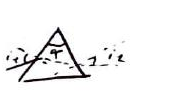
\includegraphics[width=.23\linewidth]{ottica_tex_assets/b36_p60_1.png}\end{center}
\subsubsection*{Specchio}
\[
\frac1p-\frac1q=-\frac2R,\qquad I=-\frac qp.
\]
\subsubsection*{Diottro}
\[
\frac{n_1}{p}+\frac{n_2}{q}=\frac{n_2-n_1}{R},\qquad
I=\frac{n_1}{n_2}\frac qp.
\]
\subsubsection*{Lenti}
\[
\frac1p+\frac1q=\frac1f,\qquad I=\frac qp.
\]
\[
\delta=k(r_1-r_2)=\frac{2\pi}{\lambda}d\sin\theta,
\]
\[
I_P(\theta)=I_0\left[\frac{\sin(N\delta/2)}{\sin(\delta/2)}\right]^2
\xrightarrow{N=2}I_P(\theta)=4I_0\cos^2\frac\delta2.
\]
\[
\sin\theta=m\frac\lambda d\quad\text{max principali},\qquad
\sin\theta=m'\frac\lambda{Nd}\quad\text{min},\qquad
\sin\theta=\left(m''+\frac12\right)\frac\lambda{Nd}\quad\text{max secondari}.
\]
% Pagina originale 61
\pagina{61}
\subsubsection*{Diffrazione}
\[
I_P=I_{\max}\left[\frac{\sin(\frac\pi\lambda a\sin\theta)}
{\frac\pi\lambda a\sin\theta}\right]^2.
\]
Massimo visibile: $\sin\theta=1$ ($\theta=\pi/2$).
\subsubsection*{Interferenza e diffrazione}
\[
I_P=I_{\max}
\underbrace{\left(\frac{\sin(\frac\pi\lambda a\sin\theta)}
{\frac\pi\lambda a\sin\theta}\right)^2}_{\text{diffrazione}}
\underbrace{\left(\frac{\sin(\frac\pi\lambda Nd\sin\theta)}
{\sin(\frac\pi\lambda d\sin\theta)}\right)^2}_{\text{interferenza}}.
\]
\[
\sin\theta=m\frac\lambda d<\frac\lambda a
\quad\Longrightarrow\quad m<\frac da\qquad\text{per essere visibile}.
\]
